\chapter{Introduction}
\label{chap:introduction}
%%%%%%%%%%%%%%%%%%%%%%%%%%%%%%%%%%%%%%%%%%%%%%%%%%%%%%%%%%%%%%%
% OUTLINE FOR INTRODUCTION 
% 1. Quick introduction of topic
    % 1.1. Traditional methods of identifying probelmatic data
    % 1.2. Machine Learning applied to more and more mundane tasks
% 2. Problem statement
    % 2.1. What is the problem?
    % 2.2. Why is it important?
% 3. Scope
    % 3.1. What is the current landscape? 
    % 3.2. How does this fit into that landscape
% 4. Objectives
    % 3.1. What does this add to the current landscape?
% 5. Structure of the thesis
    % 5.1. What is the structure of the thesis?
%%%%%%%%%%%%%%%%%%%%%%%%%%%%%%%%%%%%%%%%%%%%%%%%%%%%%%%%%%%%%%%

%% Segev Outline for Introduction
% 
% SN classification & Identification: Why important?
% Spectra as "gold standard" for classifiers 
% Attempt at spectroscopic classification
% Madgwich et al, Gravr et al (2013), Bovan et al, Mathukrishna et al (2019)
% AI/ ML approach: why better, possibly? 
% What problems does it solve
% what will you be looking at 
% i.e. de-redshifted vs not, subtypeclassification vs none, etc.
% "We will explore the following questions:

% SYB Comments:
% - There is a long history of naked-eye observations of supernovae that predates the invention of the telescope. The most well-known is probably SN 1054, which we now observe as the Crab Nebula.
% - Despite millennia of observations, the nature of these explosions was not really understood until the 1930s. It might be interesting to discuss why.
% - You don't explain what supernovae are: the end stage of the life-cycle of a massive star (usually $$>8 M_\odot$). More rarely (about 1/3 of the time) they are explosions in binary systems involving one WD star + a massive companion sharing a stellar envelope.
% - You can work these facts in, with sufficient citations.

When observing the night sky, viewers frequently encounter objects that 
are unexpected. Throughout history, objects appearing out of seemingly nowhere lit 
up regions of the night sky for a couple of weeks, only to disappear back 
into the faint glow of the surrounding stars. 
In 1885 and 1895, two of these objects came into view as astronomers gazed upwards 
for first time through telescopes, unable to definitively identify their 
origin \parencite{deVaucouleurs1985, Schaefer1995}.
These objects were eventually named `supernovae' (SNe) by Walter Baade and Fritz Zwicky, 
who were the first to suggest that these events were the cataclysmic death of stars, 
and predicted the remaining object to be a cold, 
neutron star \parencite{Baade1934}. Since then, astronomers 
have defined SNe to be the result of either the core-collapse of stars with a mass $>8M_\odot$, 
or a thermonuclear explosion in binary star systems involving a white dwarf sharing a stellar 
envelope with a larger star \parencite{Filippenko1997}. 
SNe visually identified throughout history, dating as far back as 185 CE, have been confirmed as well 
\parencite{Zhao_2006}, the most famous of which being SN 1054, now visible as the Crab Nebula. 

\section{Supernova Classification}
\label{sec:supernova-classification}
SNe have traditionally been classified based on their spectra starting with 
\textcite{Minkowski1941}, who first classified SNe into two groups based on the
presence or absence of hydrogen lines in their spectra. This evolved into 
the current classification scheme, which is based on the presence
or absence of hydrogen and silicon in the spectra of SNe (Figure~\ref{fig:sn-classification}). 

\begin{figure}[t]
    \centering
    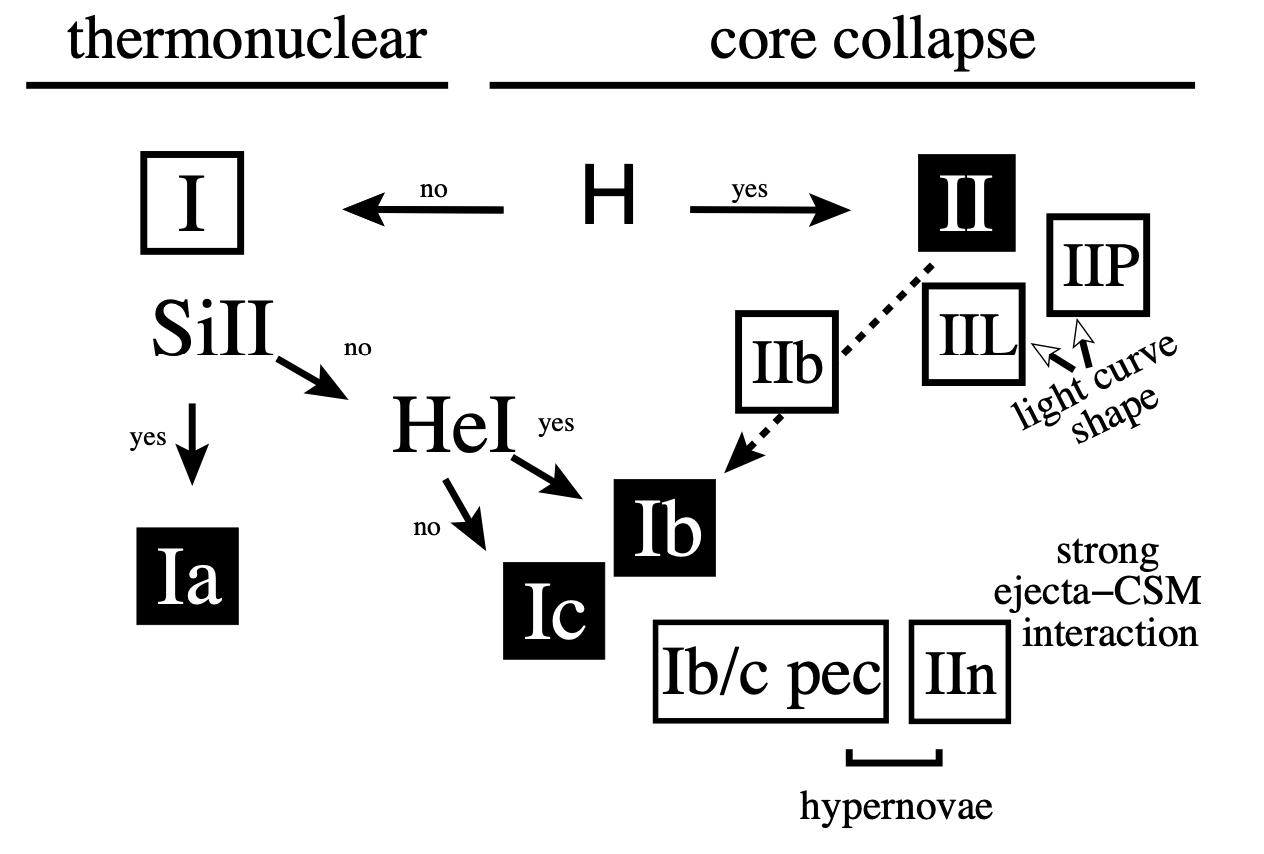
\includegraphics[width=0.8\linewidth]{figures/supernova_class.png }
    \caption[Supernova Classification]{Supernova classification. The 
    classification scheme is based on the presence or absence of hydrogen and 
    silicon features in the spectra of SNe. Figure from \textcite{Turatto2003}.}
    \label{fig:sn-classification}
\end{figure}

% The classification scheme in Figure~\ref{fig:sn-classification} is based on
% the presence or absence of hydrogen and silicon emission and absorption lines in the spectra of SNe.
SNe with hydrogen in their spectra are classified as Type II SNe, while those
without hydrogen are classified as Type I SNe. Type I SNe are further
subdivided into Type Ia, Ib, and Ic~\parencite{Turatto2003}. Although divided into three 
subtypes, Type I SNe are caused by two different mechanisms. Type Ia SNe are 
caused by the thermonuclear explosion of a white dwarf star, while Type Ib and Ic 
SNe are caused by the core-collapse of a massive star~\parencite{Filippenko1997}.
Type Ib and Ic SNe, because of this, are actually more related to Type II SNe,
and are collectively referred to as core-collapse SNe. We now know the physical
origin of the spectral differences between the subtypes: stars stripped of their 
hydrogen envelopes are appear as Type Ib SNe, while those stripped of both their 
hydrogen and helium envelopes are classified as Type Ic SNe.

% \section{Supernova Identification}
% \label{sec:supernova-identification}
Merely detecting a supernova is not enough, as astronomers must identify its
type to determine the progenitor. Traditionally, a supernova is observed by several 
means, with discovery in photometric observations and classification using follow-up 
spectroscopy (e.g. \textcite{Perlmutter1999}). This process is time-consuming, requiring not only 
the initial discovery of the supernova, but also follow-up observations to determine
the type before it fades away. Due to the large volume of new discoveries and 
the small number of single and multi-object spectrographs suitable for follow-up, only 
about 10\% of discovered SNe receive spectroscopic classification \parencite{TNS}. 
% Citation on this could be the Transient Name Server.

\section{Dark Energy Spectroscopic Instrument}
\label{sec:DESI}
% \section{Dark Energy Spectroscopic Instrument}
% \label{sec: DESI}

The Dark Energy Spectroscopic Instrument (DESI) is a spectroscopic system located in Kitt Peak 
in Arizona. Installed at the Mayall 4-m telescope, DESI is fitted with 5000 fiber roots and 10 3-arm 
spectrographs capable of resolving the [O II] $\lambda \lambda3726,3729$ doublet used for redshift
fits of galaxies \parencite{Guy2023}. This instrument is currently being used in the DESI Bright 
Galaxy Survey (BGS) to produce a map of a dark-energy dominated universe with median redshifts of $z \approx 0.2$ 
\parencite{hahn2022, desicollaboration2016}. 

Over the five year span of observations, DESI will inevitably observe SNe overlapping targets, leading to 
contaminated spectra. BGS is hypothesized to contain on order of $10^5$ supernova 
\parencite{desicollaboration2016}. An example of a supernova observed and publicly classified is shown in 
Figure~\ref{fig:desi_supernova}. Transients of any kind run the risk of influencing the redshift fit provided by DESI, 
making transient detection and identification of upmost importance to the quality of the pipeline.
The difficulties in ensuring follow-up observations of possible SNe candidates prompts the development of 
autonomous techniques geared towards the discovery and classification of these targets serendipitously. 

\begin{figure}
    \centering
    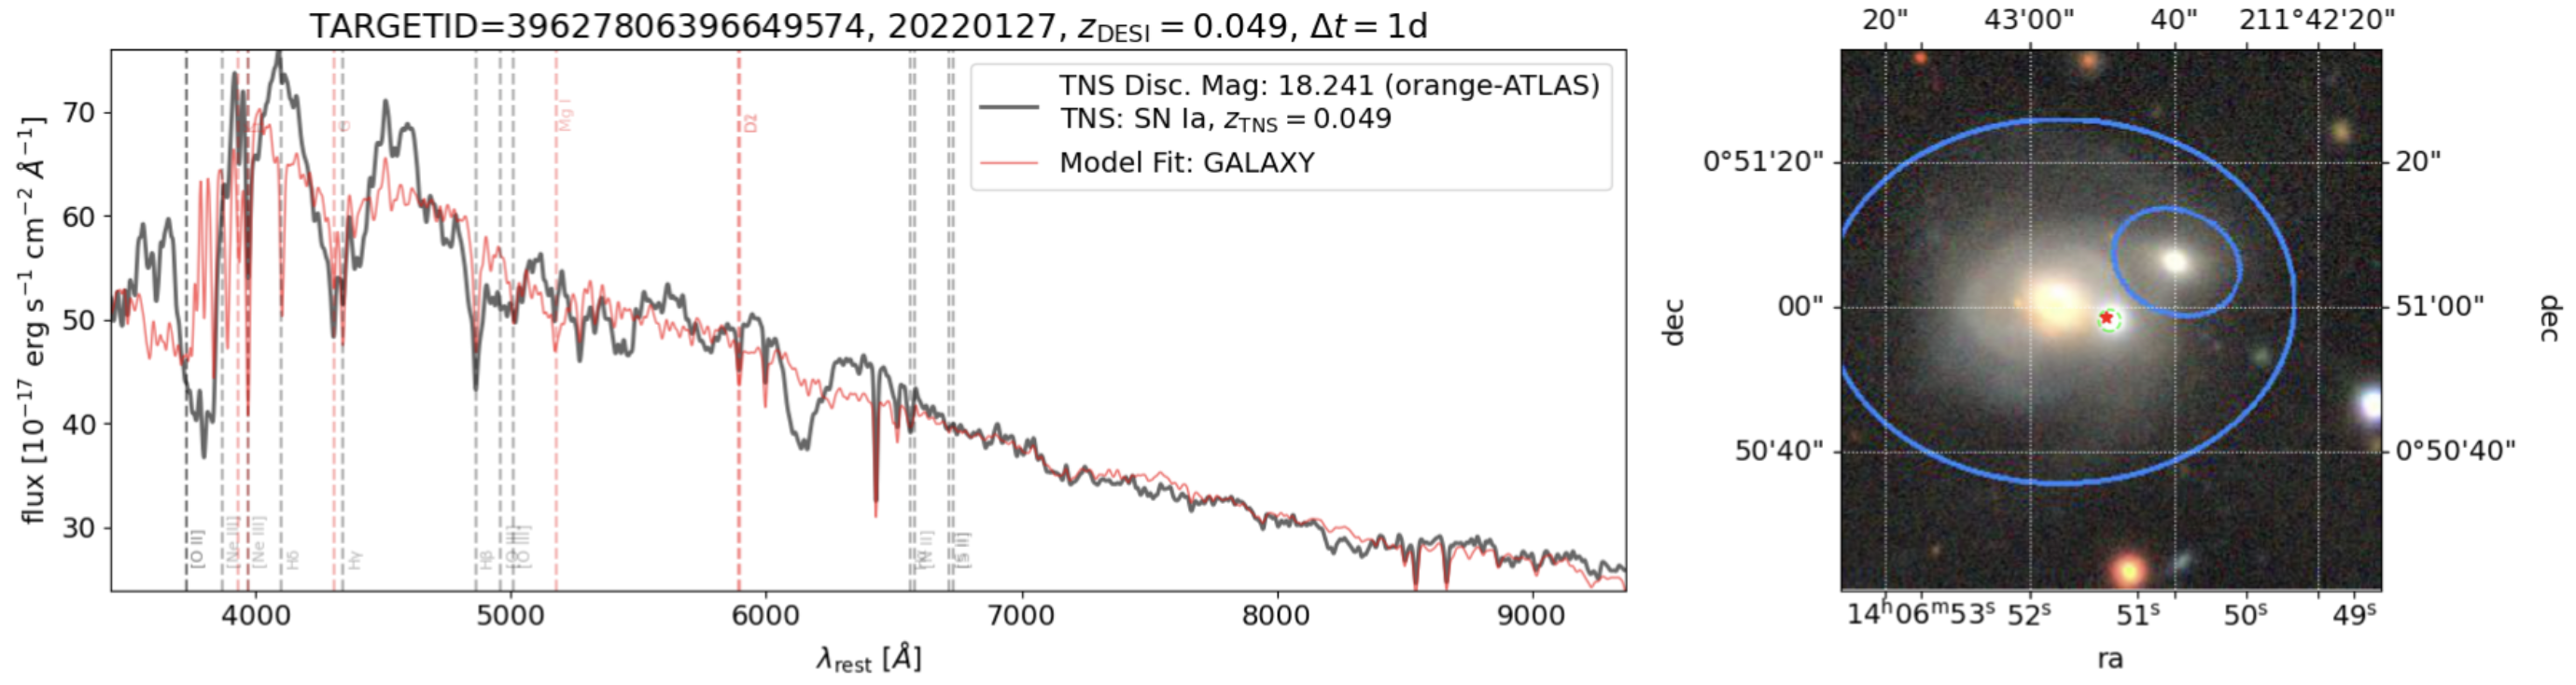
\includegraphics[width=\textwidth]{figures/desi_figures/SNe_Detection.png}
    \caption[Publicly Classified SNe captured by DESI]{DESI spectra and TNS public 
    classification of a type Ia supernova }
    \label{fig:desi_supernova}
\end{figure}

\section{Previous Approaches to Autonomous Supernova Identification}
\label{sec:PrevApproach}
The most straightforward example of an autonomous supernova identification algorithm would 
be the creation of templates for different SNe, and comparing observations against them. Raw spectra would have 
their foreground galaxies fitted and subtracted, and the residual spectrum can be identified as either background, 
or a transient.

However, this method leads to several computationally expensive issues. Firstly, the continuum 
must be accurately fitted in the presence of a possibly dominating transient. An incorrect fit 
regardless of the presence of a SNe can lead to a misclassification. Secondly, even if 
it is assumed that the residual spectrum contains only a supernova, there still needs to be 
a number of templates to be compared against. These templates must include all of the subtypes of 
SNe adjusted for all possible redshifts appropriate for the targets. In addition, the classification of 
SNe is also time dependent, so the evolution of each subtype must also be included in each template (an 
example shown in Figure~\ref{fig:sne_template}).

\begin{figure}[t]
    \centering
    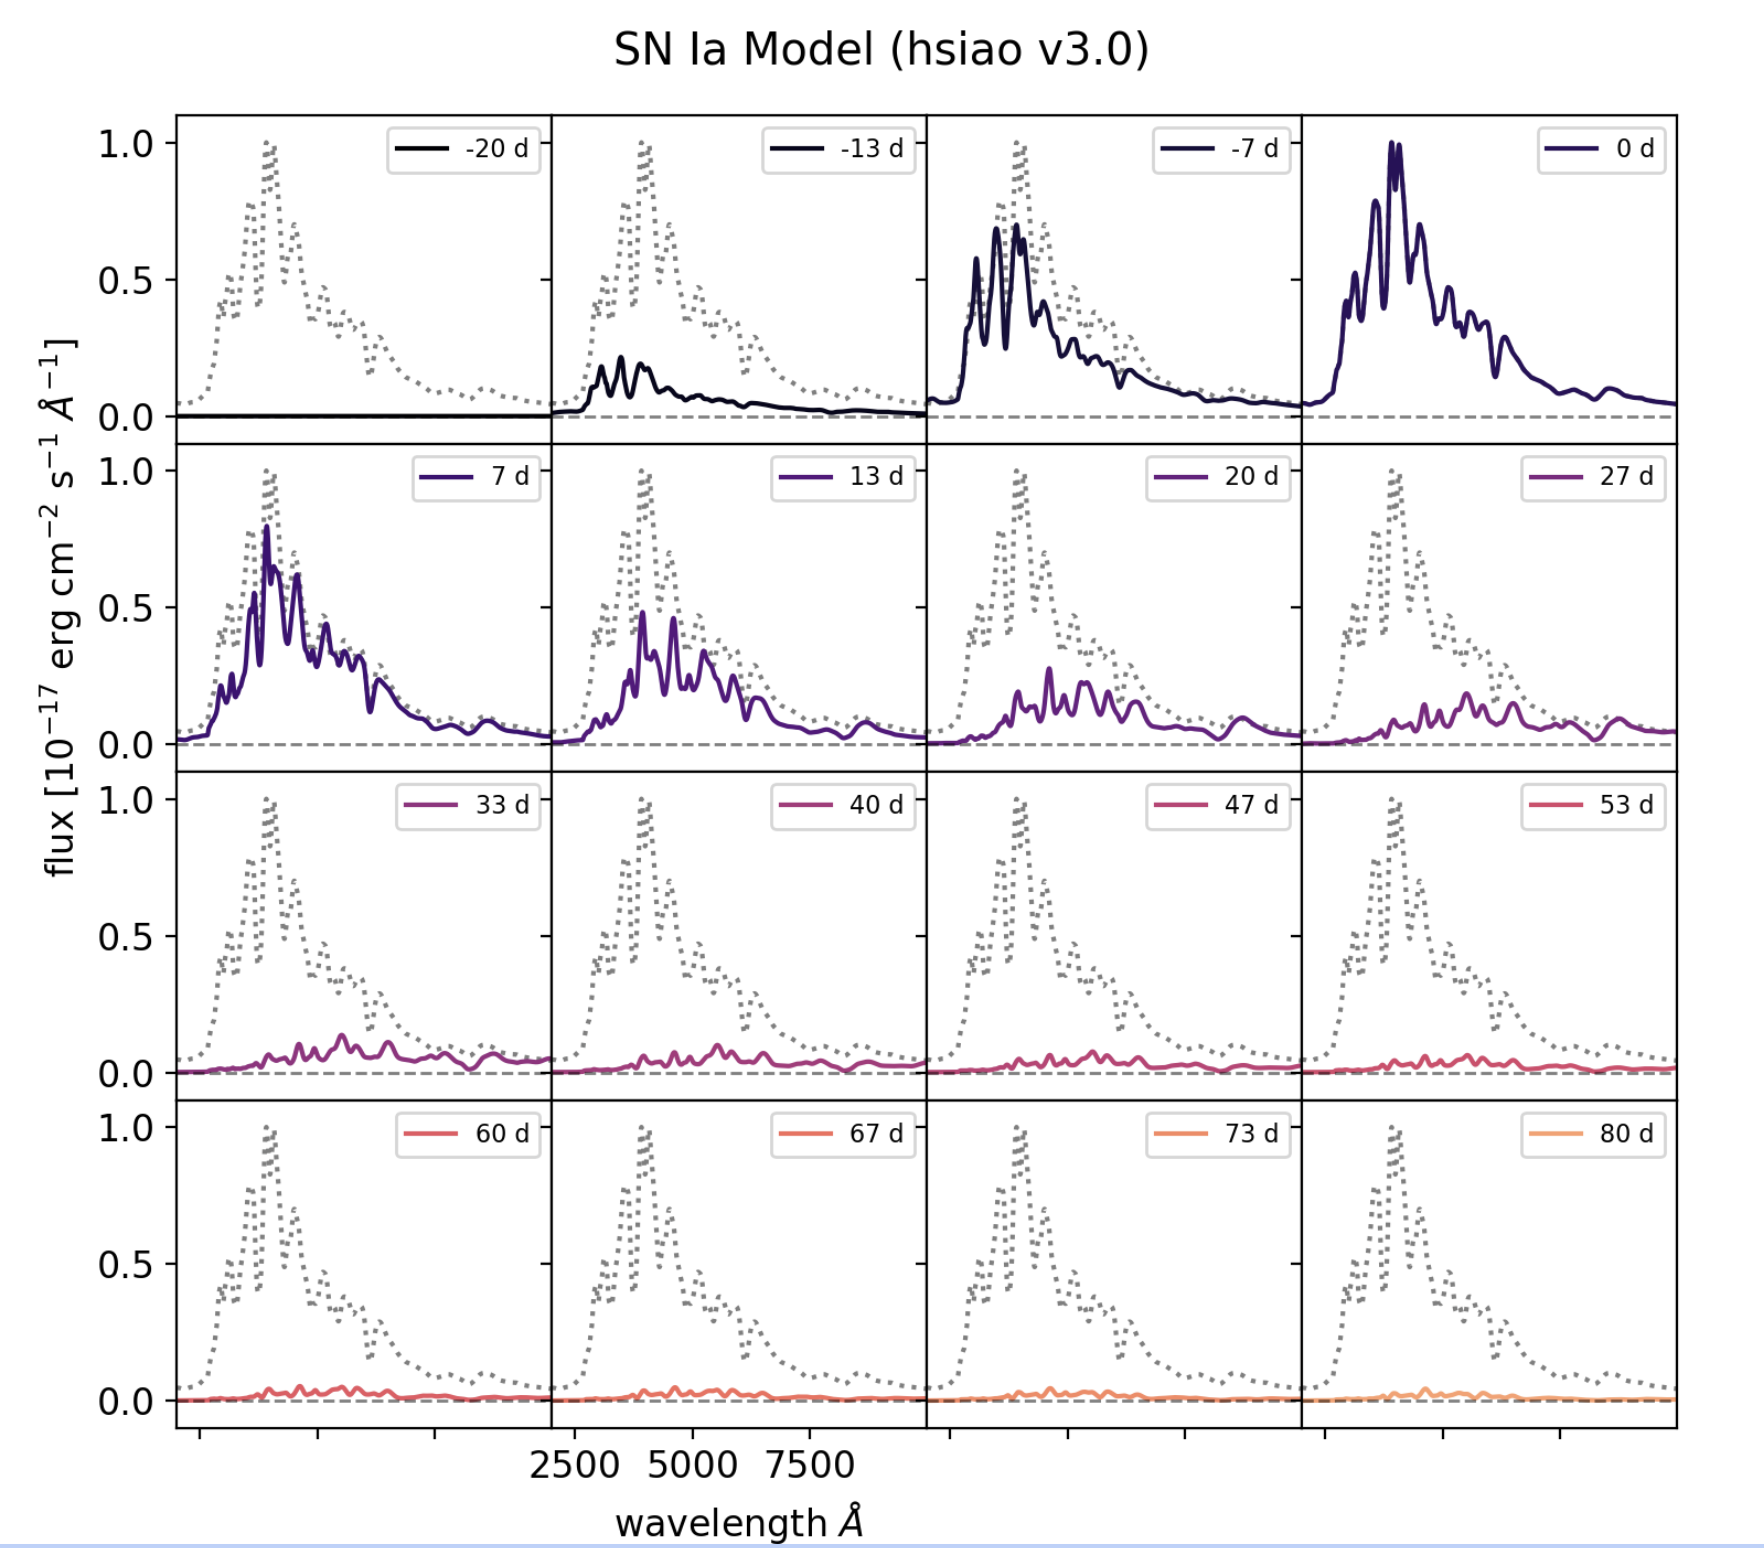
\includegraphics[width=.6\textwidth]{figures/desi_figures/snia_templates.png}
    \caption[Autonomous SNe Classification Templates]{Standard Approach to autonomous classification of 
    a type Ia supernova. Time evolution of the is shown over the course of 20 days before to 80 days after
    peak brightness. Adapted from \textcite{DESIpresentation}.}
    \label{fig:sne_template}
\end{figure}

% https://docs.google.com/presentation/d/14i0USbCQ93Mkn1T9aUK5pG24bi5bRfBhM3aVsL1Ya0U/edit?usp=sharing
% -- Look at spectra examples
% -- Look at motivation for no-redshift corrected transient classification

% https://docs.google.com/presentation/d/1zqoEVMrWbBP5k41gdjUEKioLE4J0vhu0vAzKEg4pROM/edit?usp=sharing
% -- An old presentation from 2020 that lists some past approaches to spectroscopic classification.
% -- Supernova tempates and compared them 
%   - Fit forgrown spectra from galaxy, fit residual spectrum. CHi^2 fit looks good?you discover it
% -- type IA evolution
%   - You can't just compare to one, you need to compare to A BUNCH because of time 
%   - So you want to compare to every template?? Convolve at different redshifts??
%   - SUUUPER expensive. ML/AI is just... better. 


\begin{comment}
% SB Comments:
% You want to motivate this in a couple of ways.
% 1) Because spectroscopic follow-up is tough, it's worthwhile to try to discover SNe serendipitously in spectra rather than only wait for discoveries in imaging surveys.
% 2) The issue with spectroscopic discovery is that you have potentially thousands of templates to compare against (all the different subtypes * all the variants of the subtypes * the spectral evolution of each variant * convolution vs redshift). Very computationally expensive!

% I suggest you give some background on previous approaches before jumping right into AI/ML.
% See the early slides in \href{https://docs.google.com/presentation/d/1zqoEVMrWbBP5k41gdjUEKioLE4J0vhu0vAzKEg4pROM/edit?usp=sharing}{this Google slideshow}.
\end{comment}

\section{Supernova Classification with Machine Learning}
\label{sec:supernova-classification-with-machine-learning}
Machine learning (ML) has been applied to many different fields for its flexibility 
and ability to find patterns in data. The emergence of Deep Learning (DL) has
allowed ML to be applied to more and more mundane tasks, such as image
classification~\parencite{krizhevsky2012}, speech recognition~\parencite{Nassif2019},
and natural language processing~\parencite{Mikolov2013}. ML and DL 
has also been applied to astronomy, with some success. \textcite{Gauci2010} used 
a random forest algorithm  to distinguish between spiral, elliptical, and irregular galaxies, 
and \textcite{Becker2021} used a convolutional neural network (CNN) to classify the morphology of
radio galaxies. CNNs found success in working within the DESI collaboration, with 
\textcite{parks2018} using the architecture to detect strong emission lines.  
These techniques have also been applied to the classification of SNe. 
\textcite{Mller2016} used a CNN to classify SNe into Type Ia and non-Type Ia SNe. 

Previous attempts at using machine learning algorithms for transient detection on DESI 
spectra have been conducted by \textcite{wasserman2021, Sepeku2022}. Both models were 
shown to be capable of high performance (further explained in Section~\ref{sec:CNNspectra}, 
but only after pipeline-dependent preprocessing and extensive cutting based on model certainty.
An alternative model based on the vision transformer (ViT) architecture is proposed to 
solve these short comings. Aptly named the ``Spectral ViT'', this model seeks to 
classify SNe into their respective subtypes with comparable precision and higher 
recall to previous models, without dependence on the DESI redshift fit for pre-processing. 

In Chapter~\ref{chap:DLTechniques}, the deep learning techniques used throughout the study 
are explained in detail, while Chapter~\ref{chap:methods} describes the creation and training 
of the ``Spectral ViT.'' The results of the study are discussed in Chapter~\ref{chap:results}, with 
future research and applications of this model presented in Chapter~\ref{chap:conclusions}. 


\begin{comment}
\section{Problem Statement}
This work will explore the following questions: how can we adapt novel deep learning 
techniques to classify SNe in the DESI dataset? Can we use this architecture to 
classify SNe into their respective subtypes accurately? And how can we decrease the amount of 
pre-processing required to classify these SNe accurately? In the following chapters,
we describe the Deep Learning techniques adopted to answer this problem (Ch. 2);
the training procedure for building our classification network (Ch. 3);
and the results using simulated DESI spectra that were resampled from actual 
DESI measurements performed in 2021 and 2022 (Ch. 4).
\end{comment}

